\begin{name}
	{\tenchude}
	{\tendethi}
	{\tentruong}
	{\thoigian}
\end{name}
\TN
\Opensolutionfile{ans}[ans/ans\currfilebase]
\begin{ex}%[2D1N1-1]
Hàm số $y=-x^3+3x^2+9x$ nghịch biến trên khoảng nào dưới đây?
\choice
{$(-1;3)$}
{\True $(3;+\infty)$}
{$(2;4)$}
{$(-\infty;1)$}
\loigiai{
Tập xác định $\mathscr{D}=\mathbb{R}$.\\
Ta có $y'=-3x^2+6x+9$.\\
$y'=0\Leftrightarrow x=-1$ hoặc $x=3$.\\
Bảng biến thiên.
\begin{center}
\begin{tikzpicture}
\tkzTabInit[lgt=1.5,espcl=2,deltacl=0.5]
{$x$/.6, $f'(x)$/.6, $f(x)$/1.5}
{$-\infty$,$-1$,$3$,$+\infty$}
\tkzTabLine{,-,0,+,0,-,}
\draw
(N12) node[below] (A) {$+\infty$}
(N23) node[above] (B) {$-5$}
(N32) node[below] (C) {$27$}
(N43) node[above] (D) {$-\infty$};
\draw[-stealth] (A)--(B);
\draw[-stealth] (B)--(C);
\draw[-stealth] (C)--(D);
\end{tikzpicture}
\end{center}
Vậy hàm số nghịch biến trên các khoảng $(-\infty;-1)$ và $(3;+\infty)$.
}
\end{ex}

\begin{ex}%[2D1N5-4]
\immini{Cho hàm số có đồ thị như hình vẽ bên. Số giao điểm của đồ thị hàm số đã cho với trục hoành là
\choice
{$2$}
{$0$}
{\True $3$}
{$1$}}
{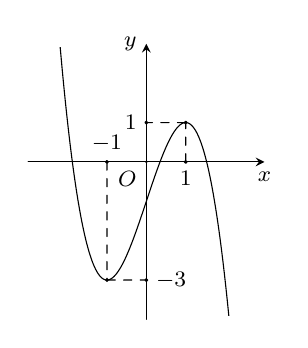
\begin{tikzpicture}[scale=0.5, font=\footnotesize, line join=round, line cap=round,>=stealth]
\def\a{-1} \def\b{0} \def\c{3} \def\d{-1}
\def\xmin{-3} \def\xmax{3}
\def\ymin{-4} \def\ymax{3}
\draw[->] (\xmin,0)--(\xmax,0) node [below]{$x$};
\draw[->] (0,\ymin)--(0,\ymax) node [left]{$y$};
\fill (0,0) circle (1.0pt) node [below left]{$O$};
\draw[dashed] (-1,0) circle (1.0pt) node [above]{$-1$}--(-1,-3)circle (1.0pt)--(0,-3) circle (1.0pt) node [right]{$-3$} (1,0)circle (1.0pt) node [below]{$1$}--(1,1)circle (1.0pt)--(0,1)circle (1.0pt) node [left]{$1$};
\clip (\xmin+0.1,\ymin+0.1) rectangle (\xmax-0.1,\ymax-0.1);
\draw[smooth,samples=300] plot(\x,{\a*(\x)^3+\b*(\x)^2+\c*(\x)+\d});
\end{tikzpicture}
}
\loigiai{
Đồ thị hàm số đã cho cắt trục hoành tại $3$ điểm.}
\end{ex}

\begin{ex}%[2-D1B4-SO-12-2425]%[VN-MT-7, VM22]%[2D1N5-1]
\immini[thm]{Cho hàm số $y=ax^3+bx^2+cx+d$ có đồ thị như hình bên.
Khẳng định nào sau đây đúng?
\choice[2]
{\True $d<0$}
{$d>0$}
{$d=0$}
{$d\leq 0$}
}{
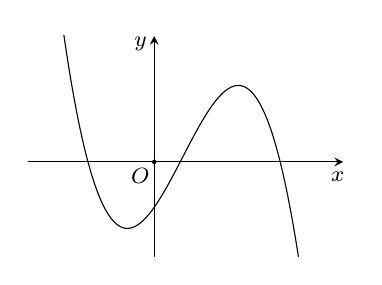
\begin{tikzpicture}[font=\footnotesize,line join=round, line cap=round, >=stealth,scale=0.8]
\def \xmin{-2}\def \xmax{3}\def \ymin{-1.5}\def \ymax{2}
\draw[->] (\xmin,0)--(\xmax,0) node[shift=(-110:0.2)] {$x$};
\draw[->] (0,\ymin)--(0,\ymax) node[shift=(-150:0.2)] {$y$};
\fill (0,0) circle(1pt) node[shift=(-135:0.25)]{$O$};
\clip (\xmin,\ymin) rectangle (\xmax,\ymax);
\draw[smooth,samples=100,domain=\xmin:\xmax] plot(\x,{-0.83*(\x)^3+1.13*(\x)^2+1.42*(\x)-0.72});
\end{tikzpicture}
}

\loigiai{
Đồ thị cắt trục tung tại điểm có tung độ âm nên $d<0$.\\
}
\end{ex}

\begin{ex}%[ID6]%[CTST-Lop12-Ontapcuoihocki1-De4]%[Bùi Lương Phúc]%[2D1N2-1]
Hàm số $y = \dfrac{x+3}{x+1}$ có bao nhiêu điểm cực trị?
\choice
{$1$}
{$3$}
{\True $0$}
{$2$}
\loigiai
{Ta có $y' = \dfrac{-2}{(x+1)^2} < 0, \, \forall x \in \mathbb{R} \setminus \{-1\}$.\\
Vì vậy hàm số không có cực trị.
}
\end{ex}

\begin{ex}%[2D1N5-1]
Bảng biến thiên trong hình dưới là đồ thị của một hàm số trong bốn hàm số được liệt kê ở bốn phương án $A, B, C, D$ dưới đây. Hỏi hàm số đó là hàm số nào?

\begin{center}

\begin{tikzpicture}
\tkzTabInit[nocadre=false,lgt=1,espcl=3]
{$x$ /1,$y'$ /1,$y$ /2}
{$-\infty$,$ -3 $,$-1$,$ 1 $,$+\infty$}
\tkzTabLine{,+,$ 0 $,-,d,-,$ 0 $,+ }
\tkzTabVar{-/ $-\infty$,+/$ -4 $,-D+ /$-\infty$/$+\infty$,-/$4$,+/$ +\infty $}
\end{tikzpicture}
\end{center}

\choice
{$y=\dfrac{x^{2}-2 x}{x+1}$}
{$y=\dfrac{x^{2}+3 x}{x+1}$}
{$y=\dfrac{1-x^{2}}{x}$}
{\True $y=\dfrac{x^{2}+2 x+5}{x+1}$}
\loigiai{
Dựa vào bảng biến thiên, ta có tiệm cận đứng $x=-1$ suy ra loại đáp án $y=\dfrac{1-x^{2}}{x}$.\\
Hàm số có điểm cực đại $(-3 ;-4)$ và cực tiểu $(1 ; 4)$ suy ra loại đáp án $y=\dfrac{x^{2}-2 x}{x+1}$ và $y=\dfrac{x^{2}+3 x}{x+1}$. Vậy đáp án $y=\dfrac{x^{2}+2 x+5}{x+1}$ đúng.
}
\end{ex}

\begin{ex}%[2D1H1-5]
Để giảm nhiệt độ trong phòng từ $28^{\circ}$C, một hệ thống làm mát được phép hoạt động trong $10$ phút. Gọi $T$ (đơn vị $^{\circ}$C) là nhiệt độ phòng ở phút thứ $t$ được cho bởi công thức $T=-0{,}008t^3-0{,}16t+28$ với $t \in[1; 10]$. Trong thời gian $10$ phút kể từ khi hệ thống làm mát bắt đầu hoạt động, nhiệt độ trong phòng tăng hay giảm?
\choice
{Tăng}
{\True Giảm}
{Tăng rồi giảm}
{Giảm rồi tăng}
\loigiai{
Xét hàm số $T=-0,008t^3-0,16t+28$ với $t \in[1; 10]$.\\
Nên $T^{\prime}=-0,024t^2-0,16< 0, \forall t \in[1; 10]$.\\
Suy ra hàm số $T$ nghịch biến trên đoạn $[1; 10]$.\\
Vậy nhiệt độ trong phòng giảm.
}
\end{ex}

\begin{ex}%[2D1N2-1]%[CD - Lớp 12 - Ôn tập cuối học kì 1 - Đề 6]%[Thơ Thơ]
Cho hàm số $y=\dfrac{x^3}{3}-2 x^2+3 x+\dfrac{2}{3}$. Toạ độ điểm cực đại của đồ thị hàm số là
\choice
{$(-1 ; 2)$}
{$\left(3 ; \dfrac{2}{3}\right)$}
{$(1 ;-2)$}
{\True $(1 ; 2)$}
\loigiai
{
Tập xác định $\mathscr{D}=\mathbb{R}$.\\
$y^{\prime}=x^2-4 x+3$.\\
$y^{\prime}=0 \Leftrightarrow x^2-4 x+3=0 \Leftrightarrow\hoac{&x=1 \\ &x=3.}$\\
Bảng biến thiên
\begin{center}

\begin{tikzpicture}
\tkzTabInit[nocadre=false,lgt=1.2,espcl=2.5,deltacl=0.6]
{$x$ /0.6,$f’(x)$ /0.6,$f(x)$ /2}
{$-\infty$,$1$,$3$,$+\infty$}
\tkzTabLine{,+,0,-,0,+,}
\tkzTabVar{-/$-\infty$,+/$2$,-/$\dfrac{2}{3}$,+/$+\infty$}
\end{tikzpicture}
\end{center}

Vậy điểm cực đại của đồ thị hàm số là $(1 ; 2)$.

}
\end{ex}

\begin{ex}%[Dự án đề ôn tập GK1, Mui Doan]%[2D1N2-2]
\immini{Cho hàm số $y=f(x)$ có đồ thị như hình vẽ bên. Mệnh đề nào dưới đây là đúng?
\choice
{Hàm số $f(x)$ đạt cực tiểu tại $x=-1$}
{Hàm số $f(x)$ đạt cực tiểu tại $x=0$}
{Hàm số $f(x)$ đạt cực đại tại $x=1$}
{\True Hàm số $f(x)$ đạt cực tiểu tại $x=1$}}
{\begin{tikzpicture}[>=stealth,line join=round,line cap=round,font=\footnotesize,scale=0.7]
\draw[->] (-2,0)--(2,0) node[right] {$x$};
\draw[->] (0,-2)--(0,4.5) node[above] {$y$};
\draw [smooth,domain=-1.1:1.8,samples=100]plot(\x,{1.5*(\x)^3-2*(\x)^2-0.5*(\x)+3});
\draw[dashed](1,0)--(1,2)--(0,2);
\fill (0,0)node[below left]{\footnotesize{$O$}}circle(1.2pt) (1,0)node[below ]{\footnotesize{$1$}}circle(1.2pt) (-1,0)node[above left]{\footnotesize{$-1$}}circle(1.2pt) (0,2)node[left]{\footnotesize{$2$}}circle(1.2pt) (0,3)node[above left]{\footnotesize{$3$}}circle(1.2pt);
\end{tikzpicture}}
\loigiai{Từ hình vẽ, ta có mệnh đề đúng là \lq\lq Hàm số $f(x)$ đạt cực tiểu tại $x=1$\rq\rq .}
\end{ex}

\begin{ex}%[Bồ Văn Hậu]%[Dự án Đề ôn thi tốt nghiệp THPT]%[2D1N4-1]
Nếu hàm số $y = f(x)$ thoả mãn $\lim\limits_{x \to -\infty} f(x) = -1$; $\lim\limits_{x \to +\infty} f(x) = 1$ thì
\choice
{Đồ thị hàm số có $2$ tiệm cận đứng là $x = -1$ và $x = 1$}
{Đồ thị hàm số có $1$ tiệm cận đứng là $x = -1$ và 1 tiệm cận ngang là $y = 1$}
{Đồ thị hàm số có $1$ tiệm cận ngang là $y = -1$ và 1 tiệm cận đứng là $x = 1$}
{\True Đồ thị hàm số có $2$ tiệm cận ngang là $y = -1$ và $y = 1$}
\loigiai{
Theo đề $\lim\limits_{x \to +\infty} f(x) = 1$ và $\lim\limits_{x \to -\infty} f(x) = -1$ nên đồ thị có hai tiệm cận ngang $y = 1$ và $y = -1$.
}
\end{ex}

\begin{ex}%[2D1N1-2]
Cho hàm số $f(x)$ có bảng biến thiên như sau
\begin{center}

\begin{tikzpicture}
\tkzTabInit[espcl=3,lgt=1,nocadre]
{$x$/0.7,$y'$/0.7,$y$/2.1}
{$-\infty$,$-1$,$0$,$1$,$+\infty$}
\tkzTabLine{,+,0,-,0,+,0,-,}
\tkzTabVar{-/$-\infty$,+/$2$,-/$-1$,+/$2$,-/$-\infty$}
\end{tikzpicture}
\end{center}
Hàm số đã cho nghịch biến trên khoảng nào dưới đây?
\choice
{$(-\infty;1)$}
{\True $(-1;0)$}
{$(-\infty;0)$}
{$(0;1)$}
\loigiai{
Từ bảng biến thên ta thấy trên khoảng $(-1;0)$ thì $f'(x) < 0$. \\
Suy ra hàm số đã cho nghịch biến trên $(-1;0)$.
}
\end{ex}

\begin{ex}%[2D1N3-1]
Đường thẳng $x = a$ được gọi là một đường tiệm cận đứng (hay tiệm cận đứng) của
đồ thị hàm số $ y = f (x)$ nếu điều kiện sau thoả mãn
\choice
{$\displaystyle\lim_{x\to +\infty }f(x)=a$}
{\True $\displaystyle\lim_{x\to a^-}f(x)=+\infty $}
{$\displaystyle\lim_{x\to -\infty }f(x)=a$}
{$\displaystyle\lim_{x\to a^-}f(x)=a $}
\loigiai{  Đường thẳng $x = a$ được gọi là một đường tiệm cận đứng (hay tiệm cận đứng) của đồ thị hàm số $ y = f (x)$ nếu ít nhất một trong các điều kiện sau thoả mãn: \\$\displaystyle\lim_{x\to a^+}f(x)=+\infty $, $\displaystyle\lim_{x\to a^+}f(x)=-\infty $, $\displaystyle\lim_{x\to a^-}f(x)=-\infty $, $\displaystyle\lim_{x\to a^-}f(x)=+\infty $.}
\end{ex}

\begin{ex}%[ID6]%[CTST-Lop12-Ontapcuoihocki1-De4]%[Bùi Lương Phúc]%[2D1N4-1]
\immini{
Cho hàm số $y = \dfrac{ax+b}{cx+d}$ (với $ad-bc \neq 0, ac \neq 0$) có đồ thị như hình vẽ. \\
Tìm phương trình đường tiệm cận đứng và ngang của đồ thị hàm số.
\choice [2]
{$x = -1, y = 1$}
{\True $x = 1, y = 1$}
{$x = 1, y = 2$}
{$x = 2, y = 1$}
}{
\begin{tikzpicture}[scale=0.5, font=\footnotesize, line join=round, line cap=round, >=stealth]
\clip (-4,-4) rectangle (6,6);
\draw[->] (-3.5,0) -- (5.5,0) node[below] {$x$};
\draw[->] (0,-3.5) -- (0,5.5) node[left] {$y$};
\draw[domain=1.23:5.5,smooth]
plot (\x,{(\x-2)/(\x-1)});
\draw[domain=-3.5:0.77,smooth]
plot (\x,{(\x-2)/(\x-1)});
\draw (-3.5,1) -- (5.5,1) (1,-3.5)--(1,5.5);
\node[below left] at (0,0) {$O$};
\node[below left] at (0,1) {$1$};
\node[left] at (0,2) {$2$};
\node[below right] at (1,0) {$1$};
\node[below] at (2,0) {$2$};
\foreach \x/\y in {0/2, 2/0} {
\fill (\x, \y) circle (1pt);
}
\fill (2,0) circle (1pt) ;
\fill (0,2)circle (1pt);
\end{tikzpicture}
}
\loigiai
{
Từ đồ thị hàm số ta có đường tiệm cận đứng là $x = 1$ và tiệm cận ngang là $y = 1$.
}
\end{ex}
\TNTF
 \begin{ex}%[2D1H5-8]
Một người chèo thuyền từ điểm $A$ trên bờ một con sông thẳng, rộng $3$ km và muốn đến điểm $B$, cách bờ đối diện $8$ km về phía hạ lưu, càng nhanh càng tốt( Hình bên dưới). Người ấy có thể chèo thuyền qua sông đến điểm $C$ rồi chạy bộ đến $B$, hoặc anh ta có thể chèo thẳng đến $B$, hoặc có thể chèo thuyền đến điểm $D$ nào đó giữa $C$ và $B$ rồi chạy bộ đến $B$. Biết rằng tốc độ chèo thuyền của người này là $6$ km/h và tốc độ chạy bộ là $8$ km/h. Biết tốc độ dòng nước là không đáng kể so với tốc độ chèo thuyền của người đàn ông.
\begin{center}
\begin{tikzpicture}[declare function={r=3;},>=stealth]
\foreach \i  in {0.2,0.6,...,8}
{\draw[ultra thin,cyan,dash pattern=on 4pt off 4pt] (0,\i)--(r,\i);}
\foreach \i   in {0,0.4,0.8,...,8}
{\draw[ultra thin,cyan,dash pattern=on 4pt off 4pt,dash phase=4pt]
(0,\i)--(r,\i);}
\draw[<->] (0,{8-0.7})--+(r,0) node[above,pos=0.5]{$3$ km};
\path (0,7) coordinate (A)
(r,7) coordinate (C)
(r,3) coordinate (D)
(r,0.25) coordinate (B);
\foreach \x in {C,D,B}{
\draw[->] (A)--(\x) node[right]{$\x$};
}
\path (A) node[left]{$A$}
(C)--(B)--([turn]90:0.75) coordinate (xt)
($(C)-(B)+(xt)$) coordinate (yt);
\draw[>=stealth,|<->|] (xt)--(yt) node[fill=white,inner sep=0pt,midway,sloped]{$8\ \mathrm{km}$};
\end{tikzpicture}
\end{center}
Gọi $x$ (km) là độ dài quãng đường $CD$. Xét tính đúng, sai của các phát biểu sau
\choiceTF[t]
{\True $8-x$ (km) là độ dài quãng đường $BD$}
{Thời gian chèo thuyền trên quãng đường $AD$ là $\dfrac{\sqrt{x^2+9}}{3}$ (giờ)}
{Tổng thời gian di chuyển từ $A$ đến $B$ là $\dfrac{\sqrt{x^2+9}}{3}+\dfrac{8-x}{8}$}
{$1$ giờ $30$ phút là khoảng thời gian ngắn nhất người này có thể đi từ $A$ đến $B$}
\loigiai{
\begin{itemchoice}
\itemch Gọi $x=CD$, với $x\in[0,8]$.\\
$\Rightarrow BD=8-x$ (km).
\itemch Thời gian người đó di chuyển từ $A$ đến $D$ là $\dfrac{\sqrt{3^2+x^2}}{6}=\dfrac{\sqrt{9+x^2}}{6}$.
\itemch Thời gian người đó di chuyển từ $D$ đến $B$ là $\dfrac{8-x}{8}.$\\
Thời gian người đó di chuyển từ $A$ đến $B$ là $\dfrac{\sqrt{9+x^2}}{6}+\dfrac{8-x}{8}$.
\itemch Thời gian người đó di chuyển từ $A$ đến $B$ là $f(x)=\dfrac{\sqrt{9+x^2}}{6}+\dfrac{8-x}{8}\cdot$\\
Khảo sát sự biến thiên của hàm $f(x)$.\\
Đạo hàm của $f'(x)=\dfrac{x}{6\sqrt{x^2+9}}-\dfrac{1}{8}\cdot$\\
Phương trình $f'(x)=0$ tương đương với
\begin{eqnarray*}
& 	& 4x=3\sqrt{x^2+9}\\
&\Leftrightarrow &
\heva{&x \geq 0\\&16x^2=9 \left(x^2+9\right)} \\
&\Leftrightarrow & x=\dfrac{9\sqrt{7}}{7}.
\end{eqnarray*}
Bảng biến thiên
\begin{center}
\begin{tikzpicture}[font=\normalsize,t style/.style={style=solid}]
%dòng khai báo
\tkzTabInit[nocadre=true,lgt=1.2,espcl=2.5,deltacl=0.5]
{$x$ /0.75, $y'$/0.75, $y$/2.5}
{$-\infty$, $0$, $\dfrac{9\sqrt{7}}{7}$, $8$, $+\infty$}
%dòng xét dấu
\tkzTabLine{,, , -,0,+,,, } % z, t, d;
%dòng biến thiên
\fill[pattern=north east lines] (T11)--(N21)--(N23)--(T13)--cycle;
\fill[pattern=north west lines] (T21)--(N41)--(N43)--(T23)--cycle;
\draw (N21)--(N23) (N41)--(N43);
\path
($(N22)!0.215!(N23)$) node[fill=white,inner sep=1pt] (A2){$\dfrac{3}{2}$}
($(N32)!0.85!(N33)$) node (A3){$\dfrac{\sqrt{7}}{8}+1$}
($(N42)!0.215!(N43)$) node[fill=white,inner sep=1pt] (A4){$\dfrac{\sqrt{73}}{6}$};
\foreach \x/\y in {A2/A3,A3/A4}{
\draw[-stealth] (\x)--(\y);
}
\end{tikzpicture}
\end{center}
Dựa vào bảng biến thiên ta thấy thời gian ngắn nhất để di chuyển từ $A$ đến $B$ là $1+\dfrac{\sqrt{7}}{8} \approx 1$ giờ $20$ phút.\\
\end{itemchoice}
}
\end{ex}

\begin{ex}%[2D1V3-6]%[Tran Ngoc Thanh]%[Du an C]
	Giả sử chi phí để xuất bản $x$ cuốn tạp chí (gồm: lương cán bộ, công nhân viên, giấy in,...) được cho bởi công thức sau:
	$C(x)=0{,}0001x^2-0{,}2x+10000$
	trong đó $C(x)$ được tính theo đơn vị là vạn đồng. Chi phí phát hành cho mỗi cuốn là $4$ nghìn đồng.
	Xét tính đúng sai của các khẳng định sau
	\choiceTF
	{Chi phí để xuất bản $100$ cuốn tạp chí là $980$ vạn đồng}
	{Tổng chi phí $T(x)$ (xuất bản và phát hành) cho $100$ cuốn tạp chí là $1200$ vạn đồng}
	{\True Chi phí trung bình $M(x)=\dfrac{T(x)}{x}$ khi xuất bản $10000$ cuốn là $2{,}2$ vạn đồng}
	{\True Nếu nhu cầu xuất bản không quá $30000$ cuốn thì khi xuất bản $10000$ cuốn, chi phí trung bình là thấp nhất}
	\loigiai{
		\begin{itemchoice}
			\itemch Chi phí để xuất bản $100$ cuốn tạp chí là
			\[C(100)=0{,}0001\cdot 100^2-0{,}2\cdot 100+10000=981\ \text{(vạn đồng).}\]
			\itemch Chi phí phát hành cho mỗi cuốn là $4$ nghìn đồng, tức là $0{,}4$ vạn đồng.\\
			Suy ra chi phí phát hành cho $x$ cuốn là $0{,}4x$ (vạn đồng).\\
			Theo đề bài, ta có tổng chi phí xuất bản và phát hành cho $100$ cuốn tạp chí là:
			\[T(100)=C(100)+0{,}4\cdot 100=1021\;\text{(vạn đồng)}.\]
			\itemch
			Ta có $M(x)=\dfrac{T(x)}{x}=0{,}0001x+0{,}2+\dfrac{10000}{x}$.\\
			Khi đó $M(10000)=\dfrac{T(10000)}{10000}=2{,}2$ (vạn đồng).
			\itemch Khảo sát sự biến thiên của hàm số $f(x)=0{,}0001x+0{,}2+\dfrac{10000}{x}$, với $x>0$ ta được bảng biến thiên
			\begin{center}
				\begin{tikzpicture}[font=\normalsize,t style/.style={style=solid}]
					%dòng khai báo
					\tkzTabInit[lgt=1.2,espcl=4,deltacl=0.7]
					{$x$ /0.75, $f^{\prime}(x)$/0.75, $f(x)$/2.5}
					{$ 0$,$ 10000 $,$ 30000 $}
					%dòng xét dấu
					\tkzTabLine{ , -,0 , +,} % z, t, d;
					%dòng biến thiên
					\path ($(N12)!0.2!(N13)$) node (A1){$+\infty $}
					($(N22)!0.8!(N23)$) node (A2){$ f\left (10000\right) $}
					($(N32)!0.2!(N33)$) node[left=-20pt] (A3){$ f(30000) $};
					\foreach \x/\y in {A1/A2,A2/A3}{
						\draw[-stealth] (\x)--(\y);
					}
				\end{tikzpicture}
			\end{center}
			Dựa vào bảng biến thiên, ta thấy giá trị của $M(x)$ nhỏ nhất khi $x=10000$.\\
			Vậy số lượng tạp chí cần xuất bản sao cho chi phí trung bình thấp nhất là $x=10000$ cuốn.
		\end{itemchoice}
	}
\end{ex}

\begin{ex}%[Dự án BG 4in1, Nguyễn Văn Nay]%[2D1H3-2]
\immini{Cho hàm số $f(x)$ liên tục trên đoạn $[-1;3]$ và có đồ thị như hình vẽ bên. Mỗi khẳng định sau đúng hay sai?
\choiceTF
{\True Hàm số có $2$ điểm cực trị trên $[-1;3]$}
{$\max\limits_{[-1;3)} f(x)=3$}
{$\min\limits_{[-1;2]} f(x)=2$}
{Giá trị lớn nhất của hàm số $y=g(x)=f\left(3|\cos x|-1 \right)$ bằng $3$}
}{
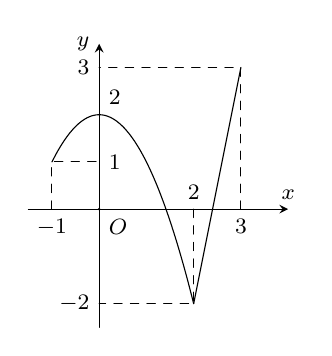
\begin{tikzpicture}[scale=0.6,line join=round, line cap=round,smooth,font=\footnotesize,>=stealth]
\draw[->] (-1.5,0)--(4,0)node[above]{$x$};
\draw[->] (0,-2.5)--(0,3.5)node[left]{$y$};
\draw [ domain=-1:2] plot (\x,{2-(\x)^2});
\fill (0,0) node[below right]{$O$}circle(0.03)
(-1,0)node[below]{$-1$} (0,1)node[right]{$1$}
(2,0)node[above]{$2$}  (0,-2)node[ left]{$-2$}  (0,2)node[above right]{$2$}
(3,0)node[below]{$3$} (0,3)node[left]{$3$}
;
\draw (2,-2)--(3,3);
\draw[dashed](-1,0)|-(0,1)  (2,0)|-(0,-2)(3,0)|-(0,3)  ;
\end{tikzpicture}}
\loigiai{
\begin{itemchoice}
\itemch Dựa vào đồ thị, suy ra hàm số có hai điểm cực trị (điểm cực tiểu $x=2$, điểm cực đại $x=0$) trên $[-1;3]$.
\itemch Vì $f(x)\ge 3$, $\forall x\in [-1;3]$ và không tồn tại $x_0\in [-1;3)$ để $f(x_0)=3$ nên hàm số không có giá trị lớn nhất trên $[-1;3)$.
\itemch $\min\limits_{[-1;2]} f(x)=f(2)=-2$.
\itemch Đặt $t=3|\cos x|-1$, $t\in [-1;2]$.\\
Dựa vào đồ thị, ta có $\max\limits_{[-1;2]} f(t)=f(0)=2$.\\
Giá trị lớn nhất đạt được khi $t=0$, hay $\cos x=\pm \dfrac{1}{3}$.
\end{itemchoice}
}
\end{ex}

\begin{ex}%[2D1H5-7]%[DA- EX-TF-TLN2024 - Phạm Quốc Toàn]
Cho hàm số $y=x^3-3x^2+2$ có đồ thị $\left(C \right)$. Xét tính đúng sai của các phát biểu sau.
\choiceTF
{$\left(C \right)$ đi qua điểm $N \left(1; 2 \right)$}
{Có ba điểm thuộc $\left(C \right)$ có tung độ bằng $2$}
{\True $\left(C \right)$ có tâm đối xứng là $I \left(1; 0 \right)$}
{\True Tổng các hoành độ của những điểm thuộc đồ thị $\left(C \right) \colon y=x^3-3x^2+2$ cách đều hai điểm $A \left(12;1 \right)$, $B \left(-6;3 \right)$ bằng $3$}
\loigiai{
\begin{itemchoice}
\itemch {\bf Sai}. Với $x = 1 \Rightarrow y = 1^3 - 3 \cdot 1^2 + 2 =0$. Vậy điểm $N \left(1; 2 \right)$ không thuộc $\left(C \right)$.
\itemch {\bf Sai}. Xét phương trình $y=2 \Leftrightarrow x^3-3x^2+2 =2 \Leftrightarrow x^3 - 3 x^2 =0 \Leftrightarrow x=0$ hoặc $x=3$. \\
Vậy có hai điểm thuộc $\left(C \right)$ có tung độ bằng $2$.
\itemch {\bf Đúng}. Ta có $y' = 3 x^2 - 6x$ và $ y''  = 6x -6$.
\[y\rq\rq  =0 \Leftrightarrow 6x - 6 =0 \Leftrightarrow x=1 \Rightarrow y=0. \]
Vậy đồ thị $\left(C \right)$ có tâm đối xứng là $I \left(1; 0 \right)$.
\itemch {\bf Đúng}. Phương trình đường trung trực đoạn $AB$ là $x+9y-21=0$.\\
Gọi $M \left(x;y \right) \in \left(C \right)$ thỏa mãn $MA=MB$.\\
$M$ là giao điểm của đường trung trực đoạn $AB$ và đồ thị $\left(C \right)$. \\
Hoành độ các điểm $M$ là nghiệm của phương trình \\
$x^3-3x^2+2=\dfrac{21-x}{9} \Leftrightarrow 9x^3-27x^2+x-3=0 \Leftrightarrow x=3$.
\end{itemchoice}
}
\end{ex}
\TNSA
\begin{ex}%[2D1C3-6]
Một người nông dân có $15\,000\,000$ đồng với dự định làm một cái hàng rào hình chữ E dọc theo con sông (như hình vẽ) nhằm rào một khu đất có hai phần chữ nhật để trồng rau. Đối với mặt hàng rào song song với bờ sông thì chi phí nguyên vật liệu là $60\,000$ đồng một mét, còn đối với ba mặt hàng rào song song nhau thì chi phí nguyên vật liệu là $50\,000$ đồng một mét. Tìm diện tích lớn nhất của khu đất rào được.
\begin{center}
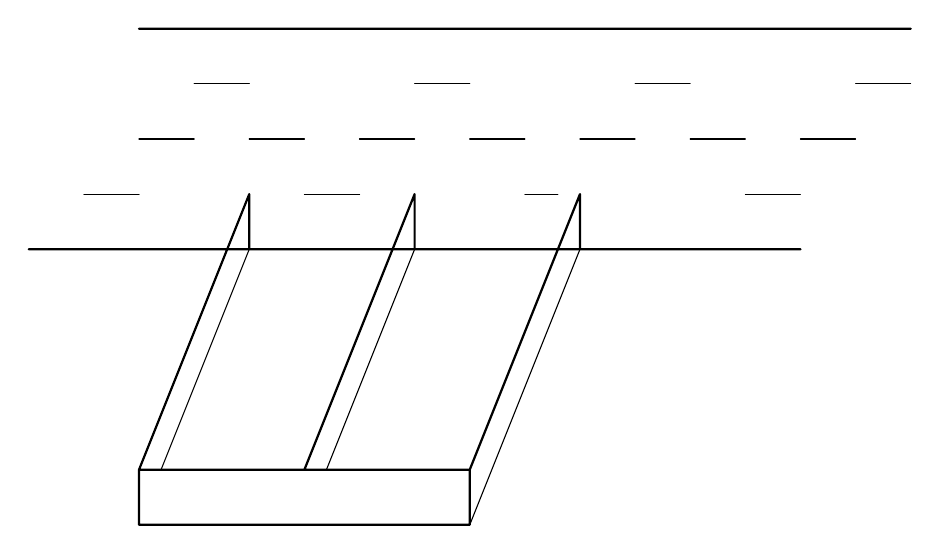
\begin{tikzpicture}[scale=0.7,>=stealth, font=\footnotesize, line join=round, line cap=round]
\draw[thick] (-4,4) -- (10,4) (-6,0) -- (8,0) (-2,0) -- (-2,1) -- (-4,-4) -- (-4,-5) -- (2,-5) -- (2,-4) -- (-4,-4) (1,0) -- (1,1) -- (-1,-4) (4,0) -- (4,1) -- (2,-4);
\draw[thin] (-2,0)--(-3.6,-4) (1,0)--(-0.6,-4) (4,0)--(2,-5);
\draw[thin] (-3,3)--(-2,3) (1,3)--(2,3) (5,3)--(6,3) (9,3)--(10,3);
\draw[thin] (-5,1)--(-4,1) (-1,1)--(0,1) (3,1)--(3.6,1) (7,1)--(8,1);
\draw[thin] (-4,2)--(-3,2) (-2,2)--(-1,2) (0,2)--(1,2) (2,2)--(3,2) (4,2)--(5,2) (6,2)--(7,2) (8,2)--(9,2);
\end{tikzpicture}
\end{center}
\shortans{$6250$}
\loigiai
{
Ta đặt kích thước của hàng rào như hình vẽ.
\begin{center}
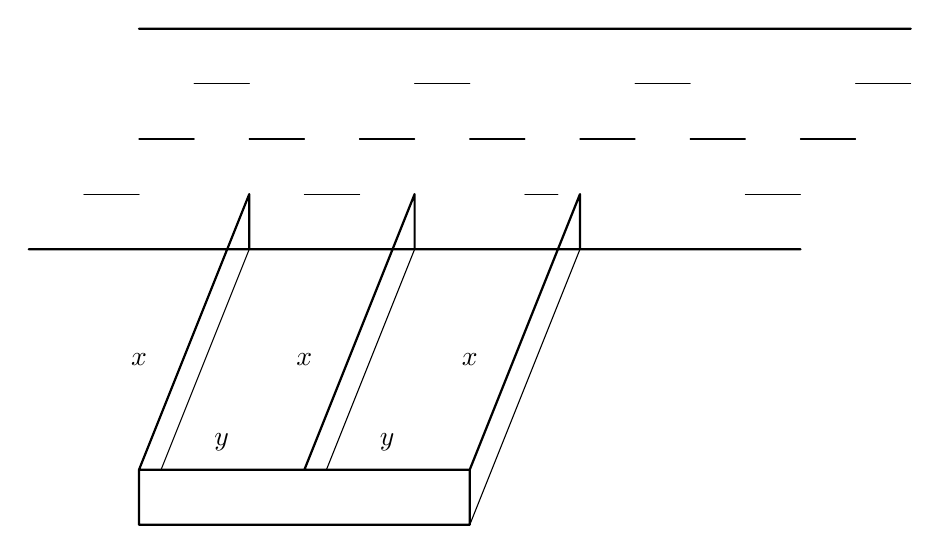
\begin{tikzpicture}[scale=0.7,>=stealth, line join=round, line cap=round]
\draw[thick] (-4,4) -- (10,4) (-6,0) -- (8,0) (-2,0) -- (-2,1) -- (-4,-4) -- (-4,-5) -- (2,-5) -- (2,-4) -- (-4,-4) (1,0) -- (1,1) -- (-1,-4) (4,0) -- (4,1) -- (2,-4);
\draw[thin] (-2,0)--(-3.6,-4) (1,0)--(-0.6,-4) (4,0)--(2,-5);
\draw[thin] (-3,3)--(-2,3) (1,3)--(2,3) (5,3)--(6,3) (9,3)--(10,3);
\draw[thin] (-5,1)--(-4,1) (-1,1)--(0,1) (3,1)--(3.6,1) (7,1)--(8,1);
\draw[thin] (-4,2)--(-3,2) (-2,2)--(-1,2) (0,2)--(1,2) (2,2)--(3,2) (4,2)--(5,2) (6,2)--(7,2) (8,2)--(9,2);
\draw (-4,-2) node {$x$} (-1,-2) node {$x$} (2,-2) node {$x$};
\draw (-2.5,-3.5) node {$y$} (0.5,-3.5) node {$y$};
\end{tikzpicture}
\end{center}
Do bác nông dân trả $15\,000\,000$ đồng để chi trả cho nguyên vật liệu và đã biết giá thành từng mặt nên ta có mối quan hệ\\
$3x \cdot 50\,000 + 2y \cdot 60\,000 = 15\,000\,000 \Leftrightarrow 15x + 12y = 1500 \Leftrightarrow y = \dfrac{1500 -15x}{12} = \dfrac{500 - 5x}{4}$.\\
Diện tích của khu vườn sau khi đã rào được tính bằng công thức\\
$f(x)=2xy=2x\cdot \dfrac{500 - 5x}{4}= \dfrac{1}{2}\left(-5x^2 + 500x\right)$.\\
Xét hàm số $f(x)=\dfrac{1}{2}\left(-5x^2+500x\right)$ trên khoảng $(0;+\infty)$.\\
Ta có $f'(x)=\dfrac{1}{2}\left(-10x + 500\right), f'(x) = 0 \Leftrightarrow x = 50$.\\
Bảng biến thiên:
\begin{center}

\begin{tikzpicture}
\tkzTabInit[nocadre=false,lgt=1.5,espcl=2,deltacl=0.6]
{$x$/0.7,$f'$/0.7,$f$/1.5}
{$0$,$50$,$+\infty$}
\tkzTabLine{,+,0,-,}
\tkzTabVar{-/$ $,+/$6250$,-/$ $}
\end{tikzpicture}
\end{center}
Vậy diện tích lớn nhất của khu đất được rào là $6250 \ (\mathrm{m}^2)$.
}
\end{ex}

\begin{ex}%[2-D1B5-SO-14-2425]%[VN-MT-7, Đỗ Minh Phúc]%[2D1V3-6]
Chị Hà dự định sử dụng hết $4$ m$^2$ kính để làm một bể cá bằng kính có dạng hình hộp chữ nhật không nắp, chiều dài gấp đôi chiều rộng (các mối ghép có kích thước không đáng kể). Bể cá có dung tích lớn nhất bằng bao nhiêu mét khối (kết quả làm tròn đến hàng phần trăm)?
\shortans{0{,}73}
\loigiai{
\begin{center}
\begin{tikzpicture}[scale=0.8, font=\footnotesize, line join=round, line cap=round, >=stealth]
\coordinate (B) at (0,0);
\coordinate (A) at (2,2);
\coordinate (C) at (4,0);
\coordinate (D) at ($(C)-(B)+(A)$);
\coordinate (B') at ($(B)+(90:3)$);
\coordinate (C') at ($(C)+(90:3)$);
\coordinate (D') at ($(D)+(90:3)$);
\coordinate (A') at ($(A)+(90:3)$);
\draw (A')--(B')--(C')--(D')--(A') (B)--(B') (C)--(C') (D)--(D')node[right,midway]{$h$} (B)--(C)node[below,midway,sloped]{$2x$}--(D)node[right,midway]{$x$};
\draw [dashed] (B)--(A)--(D) (A')--(A);
\end{tikzpicture}
\end{center}
Giả sử bể cá có kích thước như hình vẽ, với $x$, $h>0$.\\
Theo đề bài ta có $2x^2+2xh+4xh=4 \Leftrightarrow h=\dfrac{4-2x^2}{6x}$.\\
Do $x>0$, $h>0$ nên $4-2x^2>0 \Leftrightarrow 0<x<\sqrt{2}$.\\
Thể tích của bể cá là $V=2x^2h=\dfrac{4x-2x^3}{3}=f(x)$, với $x \in\left(0;\sqrt{2}\right)$.\\
Ta có $f'(x)=\dfrac{4}{3}-2x^2$.\\
Cho $f'(x)=0 \Leftrightarrow \dfrac{4}{3}-2x^2=0\Leftrightarrow x=\dfrac{\sqrt{6}}{3}$ (vì $x>0$).\\
Bảng biến thiên
\begin{center}

\begin{tikzpicture}
\tkzTabInit[nocadre,lgt=1.2,espcl=2.5,deltacl=0.6]
{$x$/0.6,$f'(x)$/0.6,$f(x)$/2}{$0$,$\tfrac{\sqrt{6}}{3}$,$\sqrt{2}$}
\tkzTabLine{,+,0,-,}
\tkzTabVar{-/$0$,+/$\tfrac{8\sqrt{6}}{27}$,-/$0$}
\end{tikzpicture}
\end{center}
Vậy bể cá có dung tích lớn nhất bằng $\dfrac{8\sqrt{6}}{27} \mathrm{~m}^3 \approx 0{,}73 \mathrm{~m}^3$.
}
\end{ex}

\begin{ex}%[Mức độ 2]%[Dự án giảng new 4in1, Trần Quang Thạnh]%[2D1H1-3]
Có bao nhiêu giá trị nguyên của tham số $m$ để hàm số $y=\dfrac{1}{3}x^3-mx^2-4mx+1$ đồng biến trên $\mathbb{R}$?
\shortans{5}
\loigiai{
Ta có $y'=x^2-2mx-4m$.\\
Hàm số đồng biến trên $\mathbb{R}$ khi và chỉ khi $y'\geq 0$, $\forall x\in \mathbb{R}$, hay $\Delta'=m^2+4m \leq 0$, tức là $-4\leq m \leq 0$.\\
Vậy có $5$ giá trị nguyên của tham số $m$ để hàm số $y=\dfrac{1}{3}x^3-mx^2-4mx+1$ đồng biến trên $\mathbb{R}$ là $-4; -3; -2; -1; 0$.
}
\end{ex}

\begin{ex}%[2D1C4-3]
Tìm được trên đồ thị $\left( C \right)\colon y=\dfrac{x+2}{x-3}$ những điểm $M$ sao cho khoảng cách từ điểm $M$ đến đường tiệm cận đứng bằng $\dfrac{1}{5}$ khoảng cách từ điểm $M$ đến đường tiệm cận ngang. Hỏi có bao nhiêu điểm $M$ thỏa mãn?
\shortans{$2$}
\loigiai{Hàm số đã cho xác định và liên tục trên $\left( -\infty ;3 \right)\cup \left( 3;+\infty \right)$. \\
Gọi đường tiệm cận đứng, tiệm cận ngang lần lượt là $\left( d_1 \right)\colon x=3,\left( d_2 \right)\colon y=1$.\\
Ta có $M\left( x_0;y_0 \right)\in \left( C \right)\Rightarrow M\left( x_0; \dfrac{x_0+2}{x_0-3} \right)$.\\
Ta có $d\left( M,d_1 \right)=\left| x_0-3 \right|$, $d\left( M,d_2 \right)=\left| \dfrac{x_0+2}{x_0-3}-1 \right|=\left| \dfrac{5}{x_0-3} \right|$. \\
Theo bài ra ta có $\left| x_0-3 \right|=\dfrac{1}{5}\left| \dfrac{5}{x_0-3} \right|\Leftrightarrow \left( x_0-3 \right)^2=1\Leftrightarrow \hoac{& x_0=4 \\ &x_0=2.}$\\
Vậy có $2$ điểm thỏa mãn $M_1\left( 2;-4 \right),M_2\left( 4;6 \right)$.}
\noindent \textbf{Chú ý.}
\begin{enumerate}
\item $d\left( M,d_1 \right)\cdot d\left( M,d_2 \right)=\left| x_0-3 \right|\cdot \left| \dfrac{5}{x_0-3} \right|=5$.
\item $d\left( M,d_1 \right)+d\left( M,d_2 \right)\geq 2\sqrt{d\left( M,d_1 \right)\cdot d\left( M,d_2 \right)}=2\sqrt{5}$.
\end{enumerate}
\end{ex}

\begin{ex}%[2D1V4-3]
Cho hàm số $y=\dfrac{2x+1}{x-1}\quad(C)$. Tính tổng tung độ các điểm $M$ thỏa mãn $M$ thuộc đồ thị $(C)$ đồng thời khoảng cách từ $M$ đến tiệm cận đứng của đồ thị $(C)$ bằng khoảng cách từ $M$ đến trục $Ox$.
\shortans{$2$}
\loigiai{
Gọi $M\left( x;\dfrac{2x+1}{x-1} \right)\in (C)$.\\
Theo đề bài ta có $\mathrm{d}\left( M,\text{TCĐ} \right)=\mathrm{d}\left( M,Ox \right)$\\
$\Leftrightarrow \left| x-1 \right|=\left| \dfrac{2x+1}{x-1} \right|$ điều kiện $\left( x\ne 1 \right)\Leftrightarrow \left| {{\left( x-1 \right)}^{2}} \right|=\left| 2x+1 \right|$ $\Leftrightarrow \hoac{& x=0 \\ & x=4.}$\\
Có hai điểm $M_1(0;-1)$ và $M_2( 4;3)$.\\
Vậy $y_1+y_2=-1+3=2$.
}
\end{ex}

\begin{ex}%[2D1V3-2]%[CD - Lớp 12 - Ôn tập cuối học kì 1 - Đề 5]%[Đoàn Thị Lý]
Giả sử chi phí để xuất bản $x$ cuốn tạp chí (gồm: lương cán bộ, công nhân viên, giấy in,...) được
cho bởi công thức $C(x)=0{,}0001 x^2-0{,}1 x+10\,000$, trong đó $C(x)$ được tính theo đơn vị là vạn đồng ($1$ vạn đồng $=10\,000$ đồng). Chi phí phát hành cho mỗi cuốn tạp chí là $3$ nghìn đồng. Ta gọi $T(x)$ là tổng chi phí bao gổm chi phí xuất bản và chi phí phát hành cho $x$ cuốn tạp chí. Tỉ số $M(x)=\dfrac{T(x)}{x}$ được gọi là chi phí trung bình cho một cuốn tạp chí khi xuất bản $x$ cuốn. Tìm chi phí trung bình thấp nhất cho một cuốn tạp chí là bao nhiêu vạn đồng (làm tròn đến hàng phần chục), biết rằng nhu cầu hiện tại xuất bản không quá $30\,000$ cuốn?
\shortans{$2{,}2$}
\loigiai{
Chi phí phát hành cho mỗi cuốn là $3$ nghìn đồng, tức là $0{,}3$ vạn đồng.\\
Suy ra chi phí phát hành cho $x$ cuốn là $0{,}3 x$ (vạn đồng).\\
Theo đề bài, ta có tổng chi phí xuất bản và phát hành cho $x$ cuốn tạp chí là
\[
T(x)=C(x)+0,3 x=0{,}0001 x^2+0{,}2 x+10\,000 \text { với } 0<x \leq 30\,000.
\]
Xét hàm số $f(x)=M(x)=\dfrac{T(x)}{x}=0{,}0001 x+0{,}2+\dfrac{10\,000}{x}$, với $0<x \leq 30\,000$.\\
Ta có $f'(x)=0{,}0001-\dfrac{10\,000}{x^2}=\dfrac{0{,}0001 x^2-10\,000}{x^2}$, $f'(x)=0 \Leftrightarrow x=10\,000\, (\text {do } x>0)$.\\
Lại có $\lim\limits_{x \to 0^{+}} f(x)=+\infty$.\\
Bảng biến thiên của hàm số $y=f(x)$:
\begin{center}

\begin{tikzpicture}
\tkzTabInit[nocadre=true, lgt=1.2, espcl=4, deltacl=0.5]
{$x$/0.7,$f’(x)$/0.7,$f(x)$/2}
{$0$,$10\,000$,$30\,000$}
\tkzTabLine{,-,z,+,}
\tkzTabVar{+/$+\infty$,-/$f(10\,000)$,+/$f(30\,000)$}
\end{tikzpicture}
\end{center}
Dựa vào bảng biến thiên, ta thấy giá trị của $M(x)$ nhỏ nhất khi $x=10\,000$.\\
Do đó, số lượng tạp chí cần xuất bản sao cho chi phí trung bình thấp nhất là $x=10\,000$ cuốn.\\
Vậy chi phí trung bình cho một cuốn tạp chí khi xuất bản $10\,000$ cuốn là $M(10\,000)=2{,}2$ (vạn đồng).
}
\end{ex}
\Closesolutionfile{ans}
